\chapter{Progetto 2: Compressione di immagini tramite la DCT}

\section{Introduzione}
Per la realizzazione della compressione di immagini, è stato scelto di utilizzare
\href{https://julialang.org/}{\textbf{Julia}}, un linguaggio di programmazione open-source,
sviluppato per ottenere prestazioni elevate e con una sintassi ad alto livello simile
a quella di Python e MATLAB. Essendo concepito per la manipolazione efficace del
calcolo scientifico, offre una vasta gamma di librerie per la gestione di matrici,
vettori e le loro trasformazioni.

In questo progetto è stata implementata l'equazione della discrete cosine transform $2$ (DCT2).
La sua implementazione è stata realizzata applicando sequenzialmente sulla matrice
la discrete cosine transform $1$ (DCT) \textcolor{blue}{prima} per righe e poi
per colonne. \st{In questo modo è stato possibile riutilizzare più efficacemente il
    codice senza introdurre code smells}. % Dubito che sappiano cosa siano gli smell codes
\textcolor{blue}{In questo modo, è stata aumentata la riutilizzabilità del codice
    e ridotto il rischio di introdurre errori.}

\textcolor{blue}{Per effettuare il confronto è stata utilizzata la libreria Julia}
\st{La libreria della FFT di Julia utilizzata è} \href{https://github.com/JuliaMath/FFTW.jl}{FTTW}
che implementa un binding con la libreria di C, entrambe le librerie sono open source.

\section{DCT2 custom}
Come \textcolor{blue}{detto} \st{preannunciato} in precedenza, è stato necessario concentrarsi solo in una implementazione
efficiente della DCT, la \textcolor{blue}{cui} sua formula è stata riportata nell'equazione \ref{eq:dct}.

\begin{equation}
    X_k = \begin{cases}
        \sqrt{\frac{1}{N}}\cdot \sum_{n=0}^{N-1} x_n \cos\left[\frac{\pi}{N}\left(n + \frac{1}{2}\right) n \right] & k=1     \\
        \sqrt{\frac{2}{N}}\cdot\sum _{n=0}^{N-1}x_{n}\cos \left[\frac{\pi}{N}\left(n+\frac{1}{2}\right)n\right]    & k \ne 1
    \end{cases}
    \label{eq:dct}
\end{equation}

Per prima cosa \textcolor{blue}{si} è \st{stato} pensato di utilizzare un approccio basato su operazioni
tra vettori e matrice, più precisamente \textcolor{blue}{si} è \st{stato} pensato di pre-calcolare la matrice
della base dei coseni (per righe) prima di effettuare il calcolo dei coefficienti.
Successivamente si effettua un prodotto matrice-\textcolor{green}{vettore} per ottenere il vettore
dei coefficienti, infine \textcolor{blue}{si è} applica la normalizzazione su di essi.

Dato un generico vettore $X_k$, per applicare la dct si effettua:
\begin{equation*}
    dct(X_k) = norm(B_{\cos}\cdot X_k )
\end{equation*}
\textcolor{blue}{dove $\cdot$ rappresenta il prodotto matrice-vettore, $B_{\cos}$
    è la base dei coseni creata per riga e $X_k$ è il vettore colonna iniziale.
    I coefficienti così ottenuti vengono normalizzati nel seguente modo:
    \begin{itemize}
        \item Il primo coefficiente viene moltiplicato per $\sqrt{\frac{1}{N}}$
        \item I restanti vengono moltiplicati per $\sqrt{\frac{2}{N}}$
    \end{itemize}
}

\st{Dove $\cdot$ è il prodotto vettore matrice e $B_{\cos}$ è la base dei coseni creata
    per riga, mentre $X_k$ è il vettore colonna iniziale. La funzione di normalizzazione
    normalizza i coefficienti del vettore risultante nel seguente modo, normalizza
    per $\sqrt{\frac{1}{N}}$ il primo coefficiente, mentre gli altri li normalizza
    per $\sqrt{\frac{2}{N}}$.
}% ! Non ho capito, normalizza per caso?

L'implementazione della DCT2 si articola nel seguente modo:
\begin{itemize}
    \item si genera la base dei coseni per riga
    \item si applica inplace la DCT1 per righe
    \item si applica inplace la DCT1 per colonne
\end{itemize}
\textcolor{blue}{Utilizzando questa strategia si riesce ad ottenere dei tempi di esecuzione}
\st{In questo modo si riescono ad ottenere dei tempi} comparabili alla DCT2 implementata
dalla libreria usando la FFT.

\subsection{Studio di complessità}
L'algoritmo custom che è stato sviluppato ha dei tempi di esecuzione comparabili
con la libreria.

La complessità della DCT2 custom è la seguente:
\begin{itemize}
    \item \textbf{generazione della base dei coseni}: \textcolor{blue}{questa operazione} \st{la generazione} richiede
          un numero costante di operazioni tra scalari e un calcolo del coseno per ogni
          entry della matrice. \textcolor{blue}{Avremo quindi}\st{Questo richiede} un totale $\mathcal{O}(N^2)$ per generare
          la matrice, quando $N\times N$ è la dimensione della matrice (dimensione dello
          spazio vettoriale per numero di coefficienti).
    \item \textbf{applicazione della DCT1 su un vettore}: \st{l'applicazione della DCT1
              su un generico vettore} richiede di effettuare un prodotto matrice-vettore e
          successivamente di normalizzare i coefficienti. Il prodotto matrice-vettore
          ha una complessità asintotica di $\mathcal{O}(N^2)$, dove $N$ è la dimensione
          del vettore. Mentre per normalizzare i coefficienti si richiede una scansione
          lineare del vettore che richiede $\mathcal{O}(N)$, dove $N$ è la dimensione
          del vettore. Quindi complessivamente si ha una complessità di $\mathcal{O}(N^2 + N) = \mathcal{O}(N^2)$.
    \item \textbf{applicazione della DCT2 sull'intera matrice}: l'applicazione della DCT2
          sull'intera matrice richiede di eseguire una DCT1 per ogni riga e poi per ogni
          colonna. All'atto pratico, non si rigenera ogni volta la matrice dei coseni,
          bensì inizialmente la si pre-calcola ($\mathcal{O}(N^2)$), successivamente si
          esegue la DCT1 per righe che richiede $\mathcal{O}(N \cdot N^2)$ ($N$ righe
          per $N^2$ la moltiplicazione riga-matrice) e successivamente si applica la
          DCT1 per colonne che richiede $\mathcal{O}(N \cdot N^2)$ ($N$ colonne
          per $N^2$ la moltiplicazione riga-matrice). Complessivamente si ottiene
          un $\mathcal{O}(N^3)$ a livello asintotico.
\end{itemize}

L'implementazione custom della DCT2 è stata confronta anche con quella ottimizzata
dalla libreria usando la FFT e nell'immagine \ref{fig:analisi_complex} si
può vedere il confronto.

% \begin{figure}[!h]
%     \centering
%     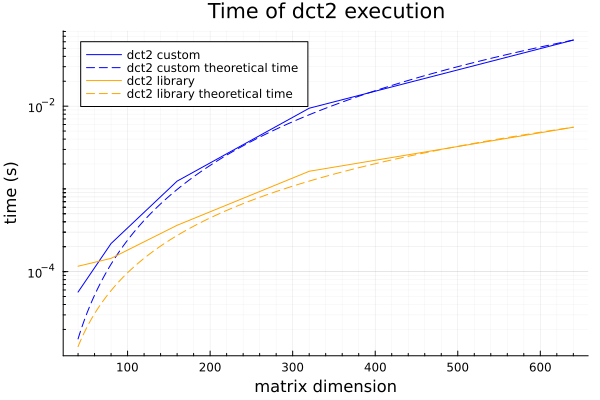
\includegraphics[width=0.5\textwidth]{Progetto_2/img/times_plot.png}
%     \caption{Grafico dei tempi al variare della dimensione della matrice. Le linee
%         continue rappresentano i dati empirici, le linee tratteggiate rappresentano
%         l'andamento teorico dei metodi.}
%     \label{fig:analisi_complex}
% \end{figure}

Come si può notare dal grafico, l'andamento empirico segue quello teorico, ovvero
la DCT custom segue $\mathcal{O}(N^3)$, mentre la DCT della libreria segue $\mathcal{O}(N^2\log N)$.

In aggiunta, parlando dello spazio occupato, la DCT custom necessita di una matrice
$N\times N$ della base dei coseni e alloca un array di dimensione $N$ per salvare
i coefficienti, quindi si ottiene una complessità spaziale di $\mathcal{O}(N^2)$.

Si può ridurre la complessità spaziale effettuando tutte le operazioni inplace.

\section{Compressione}
\textcolor{blue}{Per facilitare l'uso del software che comprime l'immagine in scala di
    grigi, si è pensato}
\st{Per l'implementazione del software che comprime l'immagine in scala di grigi, è stato
    pensato}, di sviluppare un'interfaccia mediante l'utilizzo di un framework \st{per effettuare
    data visualizzation}. Il framework scelto è un binding di \href{https://github.com/plotly/dash}{Dash} per Julia. Dash
è un framework di Python per data visualizzation interamente open source.

\subsection{Implementazione dell'interfaccia}
L'interfaccia consiste in una pagina web che chiede in input l'immagine da comprimere
e i parametri di compressione ($f$ e $d$), in output restituisce il l'immagine compressa.

Nell'interfaccia vengono mostrate entrambe le immagini, sia quella di input sia quella
compressa, in modo da confrontare la qualità delle immagini.

\subsection{Implementazione della compressione}
Dopo l'implementazione della GUI che si occupa di prendere in input l'immagine e
i due parametri, è stato sviluppato l'algoritmo di compressione dell'immagine.

L'implementazione della compressione si è articolata nel seguente modo:
\begin{itemize}
    \item \textbf{ridimensionamento dell'immagine in input}: l'immagine è stata
          ridimensionata in modo tale da avere altezza e larghezza multiple del
          parametro $f$.
    \item \textbf{implementazione della compressione}: la compressione è stata
          implementata applicando sui sotto-quadrati $f\times f$ dell'immagine
          la DCT2 della libreria, successivamente sono state azzerate le entry
          $M[k,l]$ tali che $k+l\ge d$, infine si applica IDCT2 della libreria e
          si normalizzano i valori.
    \item \textbf{visualizzazione output}: infine viene visualizzato l'output
          messo a confronto con l'input.
\end{itemize}

Nel dettaglio, la \textbf{ridimensionamento dell'immagine in input} elimina le ultime
righe e le ultime colonne dell'immagine in input in modo da avere le dimensioni
multiple di $f$.

Mentre, l'\textbf{implementazione della compressione} si articola nell'allocazione
di una matrice di appoggio $C\in \mathbb{R}^{f\times f}$ che viene inizializzata
con una sotto matrice $f\times f$ dell'immagine che si vuole elaborare. Successivamente
si applica la DCT2 della libreria, si azzerano i coefficienti $C_{kl}$ tali che
$k+1\ge d$, in seguito si applica la IDCT2 della libreria, infine si arrotondano
all'intero più vicino i coefficienti e si riportano i valori superiori a $255$
e inferiori a $0$ nell'intervallo $[0,255]$. Infine, si copia la sotto-matrice di
appoggio nell'immagine. Questo passo viene ripetuto in tutta l'immagine suddividendola
in blocchi $f\times f$ disgiunti.